% !TEX root = ../../thesis.tex

\chapter{Introduction}

In recent decades, the rise of smart interconnected devices not only changed how we interact with information, but also introduced all-new ways of engaging with the world. The rise of smartphones enabled users to consume content and perform tasks on-the-go, tablets made people rethink the ways they work and travel, wearable devices made new sets of data available to the users and so on. Ericsson Mobility Report of February 2021 reveals that the number of connected devices has been steadily increasing ~\cite{EricssonMobility2020}, and with new devices and form-factors underway, such as smart glasses, smart vehicles and folding displays, this trend is likely to continue in the foreseeable future. 

The increasing demand in the diversity of devices and device families also increased the demand for front-end application development, as it became more challenging and costly to have a decent user-facing online presence. This lead to advancements in front-end development; emerging new tools, techniques, frameworks, libraries, and SDKs made it possible to build consumer-facing products in ways that were never possible before. Nevertheless, the ever-growing front-end ecosystem and high user demands forced developers to spread their focus to overwhelming levels; (Fig ~\ref{fig:num_of_frameworks_used}) a recent survey \textit{State of JavaScript} reveals that around 60\% of developers use more than one Front-end framework, and for cross-platform frameworks, it is more than 80\% ~\cite{StateOfJs2020}. This transformation did help create a large and dynamic market of consumer products, goods and services, though it did not come without some hurdles. In this thesis, we explore what these hurdles are and discuss how Intertext addresses them.

\begin{figure}
  \centering
  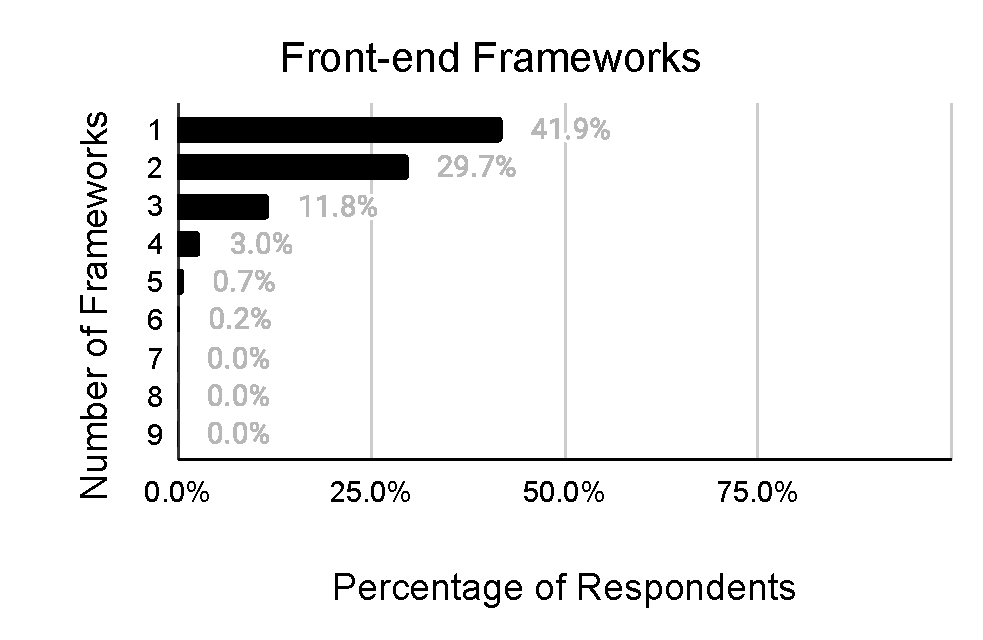
\includegraphics[width=6.2cm]{images/sojs1.pdf}
  \,
  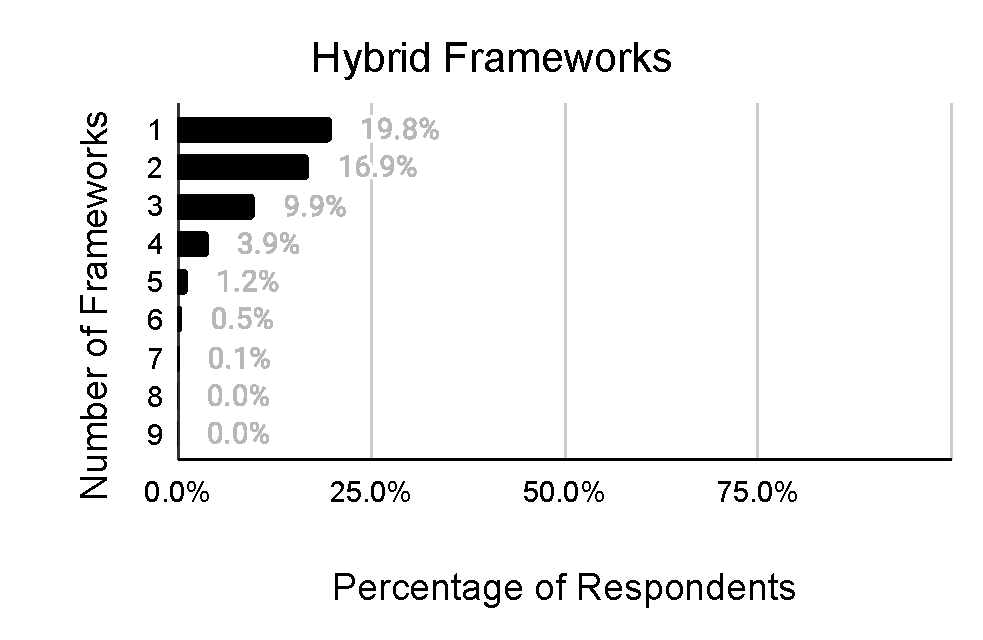
\includegraphics[width=6.2cm]{images/sojs2.pdf}
  \caption{Number of frameworks used to Percentage of respondents}%
  \label{fig:num_of_frameworks_used}%
\end{figure}

% !TEX root = ../../thesis.tex

\section{Problem Statement} \label{problemStatement}

In this thesis, we group these hurdles mentioned above under three main categories; consuming data, privacy and security, and providing data. The consuming data section discusses end-users problems due to user interface and experience inconsistencies, and lack of device and accessibility support. The Privacy and Security section argues why there are no truly private and secure environments. Providing data section gives insights into the challenges faced by data and service providers in creating front-end applications.

\subsubsection{Consuming Data}

The simplicity of consuming data is lost within the complexity of modern-day applications; nowadays, something as simple as checking the weather, reading a news article, browsing an image gallery, buying a product or service and filling out a form can be frustrating and time-consuming. One common reason for this is the inconsistencies and errors in front-end implementations. In the open market, where everyone can create user-facing applications, there is little to no enforcement or quality control measures on how a user-interface should look or how it should behave. The presentation of the same functions can significantly differ based on the implementations. For instance, some websites' navigational menu component may be on the top, and others could have it on the left or right. Some could offer hamburger-menu style functionality where the user has to click/tap on the hamburger icon to toggle on and off, but some could work by swiping gestures. Swiping gestures might toggle the navigation menu on and off, while some implementations could implement it as "go back", and so on. 

In some cases, the developer can choose a poor selection of a colour palette, causing some components to blend into the background or make it hard for users to see. Users often have to take a second to adjust to every different experience from every different provider. While some providers with higher development budgets create flawless experiences for their users, this is not always the case, and there is no guarantee.

Another major hurdle in consuming data for users is device and screen size support. Providers typically need to spend significant extra effort to support various devices and screen sizes, should they want such support in the first place. Many providers choose not to have this support to reduce development cost, leaving some users with bad experiences or no experience at all. Different levels of support for different environments might cause confusion and frustration; for instance, some providers might offer a native mobile application with native mobile gestures, while some might have a Progressive Web App (PWA) that comes with native-like gestures, and some might offer a mobile-web experience that may or may not come with smooth gestures at all. Another significant experience difference between mobile applications and web-based applications is the style of navigation. Users accustomed to using native mobile applications could expect the navigational history to retain between tabs and get frustrated when they realize that this is not the case on a mobile web application. At times improperly handled navigation in a Single Page Application (SPA) might even cause the native "back" functionality to throw the user out of the application back to the previous one.

Creating accessible front-ends is another thing that providers have to spend significant efforts on, so much so that there are even developers who specialize only in this field. Creating accessible applications is not always the priority for many development projects due to its costs and efforts. The diversity in user interfaces directly affects the accessibility aspect, as it is another implementation detail that the developer needs to deal with. There are many different ways of creating accessible user interfaces, various implementations for different kinds of accessibility needs, and different ways of implementing each one of them. For instance, in a web application, adding "focus" states to DOM elements is the most basic form of accessibility implementation that allows users to tab into a specific element to interact with it. Designing the order in which they receive focus is a whole other dimension. 

\subsubsection{Privacy and Security}

As mentioned before, there is a lack of a systematic enforcement mechanism for front-end applications. There are some protective measures in place; however, none of these measures can guarantee a completely secure and private environment ~\cite{TrackingWeb}, even the most ubiquitous browser or platform features could be used to relinquish the privacy of the users ~\cite{TrackingFavicon}. Most popular application stores typically have policies and guidelines on what the applications they distribute are allowed to do, but offending practices, especially the non-obvious ones, likely flies under the radar as most app stores do not require the source codes to be provided. Browsers and operating systems block suspicious activities to some extent, but they do not (or cannot) interfere with the legitimate (or legitimate-looking) ones. Governments implement various forms of cybersecurity laws to protect users, but laws are for the law-abiding, and as long as these laws cannot be enforced effectively, there is no safe environment for the users. As long as users are required to execute code on their devices, the bottom line is that they cannot be truly safe.

\subsubsection{Providing Data}

The word Providers refers to anyone who offers data and services to end-users, and it is safe to say that the providers also share the problems discussed under the Consuming Data section. The complexity of building a decent, well designed, accessible front-end experience, not even once but once per every client built for various platforms, forces providers to choose between supporting multiple devices, following best practices, creating a good experience. It is typically the case that providers cannot have it all initially, as it requires high costs and large teams. 

Codesharing is one of the recent trends in front-end development gaining some traction, aiming to solve some of these problems mentioned above; using react-native, react-native-web or Flutter, one can have a single codebase that produces applications for multiple environments. Modern front-end libraries/frameworks typically abstract the view layer, making it possible to create applications for different environments by swapping the view layer and wiring it up to the logic layer, which seems to be the current cross-platform application development status quo. However, the issue that comes with this approach is the difficulty in reducing the codebases for different environments into one, as it is hard to address the various requirements and features of each platform. Even though it is possible to share some extent of the code, sometimes platforms are conceptually distinct, and the software for these platforms needs to be built differently. 

Another pain point faced by providers is maintenance. The world of front-end development is an extremely fast-growing and evolving ecosystem. The changes are persistent, and at times breaking. There are thousands of tools, libraries, frameworks, SDKs available at the fingertips of developers at no cost. It is a common practice to make use of these libraries as they help with the development significantly. However, the diversity in the libraries used to build the software results in a diversity of maintenance problems. Even the most well-tested and maintained libraries could break after an update, causing a headache for the developers and hardship for the users.
% !TEX root = ../../thesis.tex

\section{Research Questions}

We have listed the problems that we are interested to solve in the section above. In light of these problems, we aim to answer the following questions in our research:

\paragraph{How can we re-imagine front-end, and improve it in such a way that:}
\begin{enumerate}
  \item from the \underline{users perspective}, for \underline{all applications} it:
  \begin{enumerate}
    \item presents a consistent User Experience (UX) ?
    \item works consistently on all supported devices and platforms ?
    \item allow users to customize the look and feel ?
    \item guarantees accessibility ?
    \item guarantees privacy ?
    \item guarantees security ?
  \end{enumerate}
  \item from the \underline{data-providers perspective}, it:
  \begin{enumerate}
    \item eliminates the need to create visually-appealing front-end applications ?
    \item eliminates the need to create accessible front-end applications ?
    \item eliminates the need to create front-end applications for every device / platform ?
  \end{enumerate}
\end{enumerate}

\paragraph{How can we create an alternate front-end realm that:}
\begin{enumerate}
  \item brings product development costs to a minimum?
  \item enables more variability of software products in the market?
  \item unifies the viewing experience, so individual developers and large companies compete on the same ground?
\end{enumerate}
% !TEX root = ../../thesis.tex

\section{Contributions} \label{contributions}

As discussed in the \nameref{problemStatement} (\ref{problemStatement}) section, Intertext ambitiously attempts to solve many different problems from various domains. A solution at this scale requires novelty, rethinking the current state of art instead of an incremental update. The biggest contribution of Intertext is to borrow existing concepts that are mostly academic and apply them to solve these real-world problems. With that said, here are some notable contributions:

\hl{TODO: combine it in new ways}

\begin{itemize}
  \item We reviewed existing research on User Interface Description Languages (UIDLs) and other similar topics to outline ways to utilise these concepts to solve the aforementioned problems.
  \item We designed IUIDL; while doing so, we decided:
  \begin{itemize}
    \item What are the concepts that are crucial to modern front-end development that needs support out-of-the-box
    \item What terminology should we use in order to create an optimal balance between the device-independent nature and developer familiarity
    \item What the syntax should be like to maximise developer friendliness
    \item How to overcome some limitation of XML in the most effective, clear and extendable way
  \end{itemize}
  \item We created an engine using Javascript / Typescript to perform common tasks of Intertext clients, such as parsing IUIDL and managing the application state
  \item We created multiple software clients that can render IUIDL into functional front-ends optimised for the host device and are user customisable where possible
\end{itemize}
% !TEX root = ../../thesis.tex

\section{Methodology}
% !TEX root = ../../thesis.tex

\section{Structure} \label{structure}

\hl{TODO: add structure}